\section{Bildschirm}
\begin{figure}[h]
    \centering
    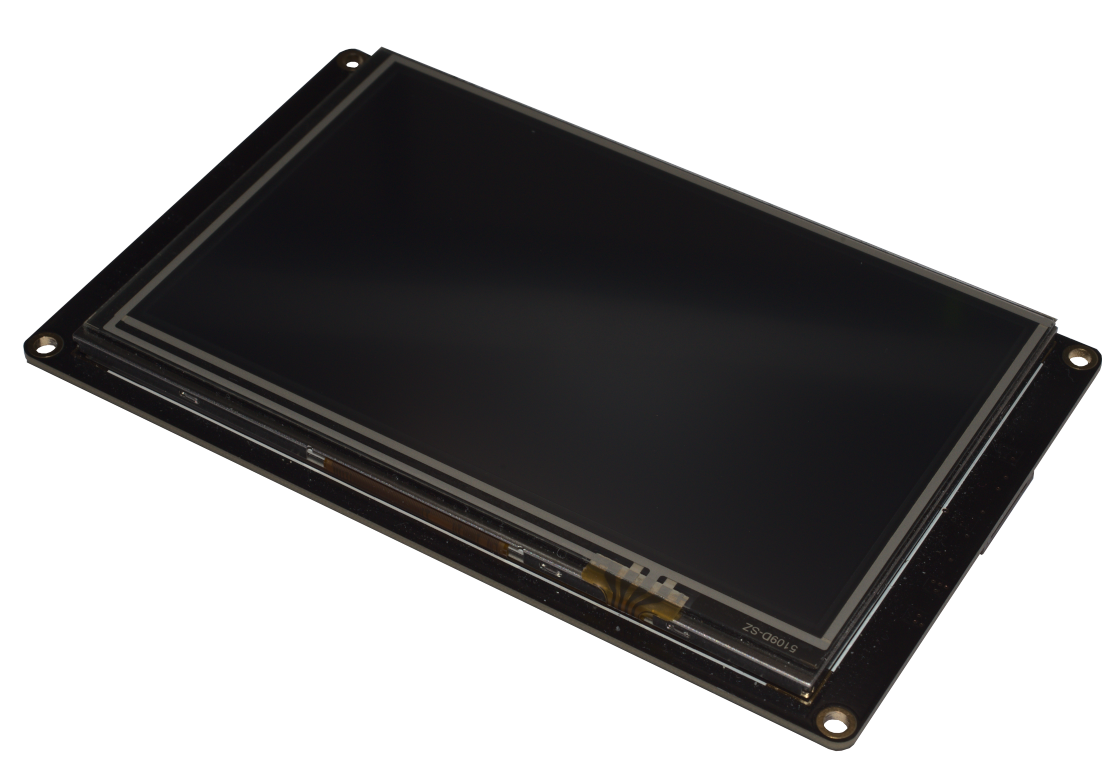
\includegraphics[width=0.8\textwidth]{Fotos/Nextion_Display.png}
    \caption{Nextion-Display}
\end{figure}
Bei dem verwendeten Bildschirm handelt es sich um einen 5 Zoll großen Touchscreen aus dem Hause Nextion.
Diese bieten den großen Vorteil, die graphische Darstellung bequem über das verfügbare gratis Tool (\textbf{Nextion Editor}) designen zu können, während der Arduino den Bildschirm nur mit den nötigen Daten über eine Serielle Verbindung versorgen muss. 

\newpage
\subsection{Installation des Nextion-Editors}
\href{https://nextion.tech/nextion-editor/}{Nextion Editor Webseite}
\begin{figure}[h]
    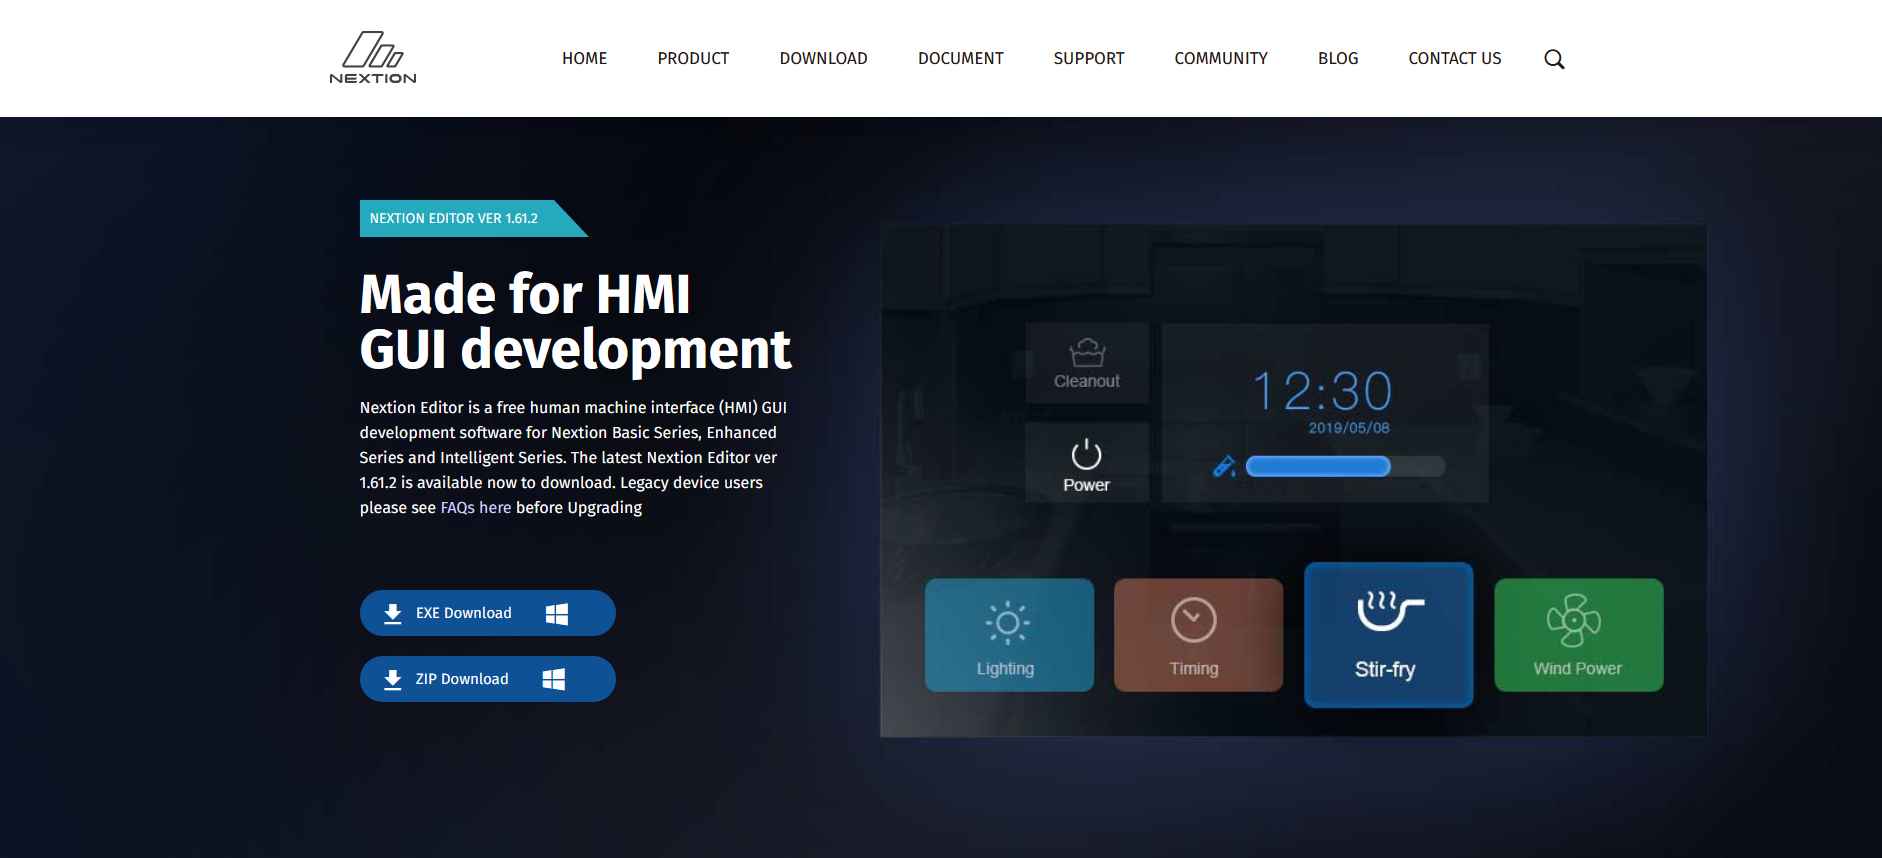
\includegraphics[width=1\textwidth]{bilder/Nextion_Webseite.png}
    \caption{}
\end{figure}